\documentclass{article}

\usepackage[margin=.75in]{geometry}
\usepackage{listings}
\usepackage{amsmath}
\usepackage{graphicx}

\lstset{
    basicstyle=\ttfamily,
    mathescape
}

\author{Damien Prieur}
\title{Homework 2 \\ CS 457}
\date{}

\begin{document}

\maketitle

Note: Sorry for the pictures being in random places, I tried to format them properly but couldn't.
I labeled which tree goes where so hopefully it's not too confusing.

\section*{Question 1}
Solve the following recurrence equation (tight upper \emph{and} lower bounds!)
\begin{equation*}
T(n)=
\begin{cases}
1 &\text{if $n< 1$}\\
2T(n/2)+23 &\text{otherwise.}
\end{cases}
\end{equation*}

\begin{itemize}
\item [a.] Using the \emph{master theorem}. Make sure to explain which case applies and why. \\
The first step for the master theorem is to identify each part and make sure it fits the form necessary.
For this equation we do match the form with coefficients
$$ a=2 \qquad b=2 \qquad f(n)=23 \quad or \quad f(n)\in O(1)$$
Lets check the first case of the master theorem
$$ f(n) \in O(n^{\log_{b}{a-\epsilon}}) $$
Plug in our numbers for $a$ and $b$
$$ 23 \in O(n^{\log_{2}{2-\epsilon}})$$
$$ \forall \epsilon \quad 1 > \epsilon > 0 \implies 0 < \log_{2}{2-\epsilon} < 1$$
$$23 \in O(n^{log_{2}{2-\epsilon}})$$
Which means we fall into the first case. By case 1 of the master theorem we have
$$ T(n) \in \Theta(n)$$


\item [b.] Using the \emph{recursion tree} method. Do not use asymptotic notation for the depth of the recursion tree; use exact upper and lower bounds instead. \\

\begin{figure}
    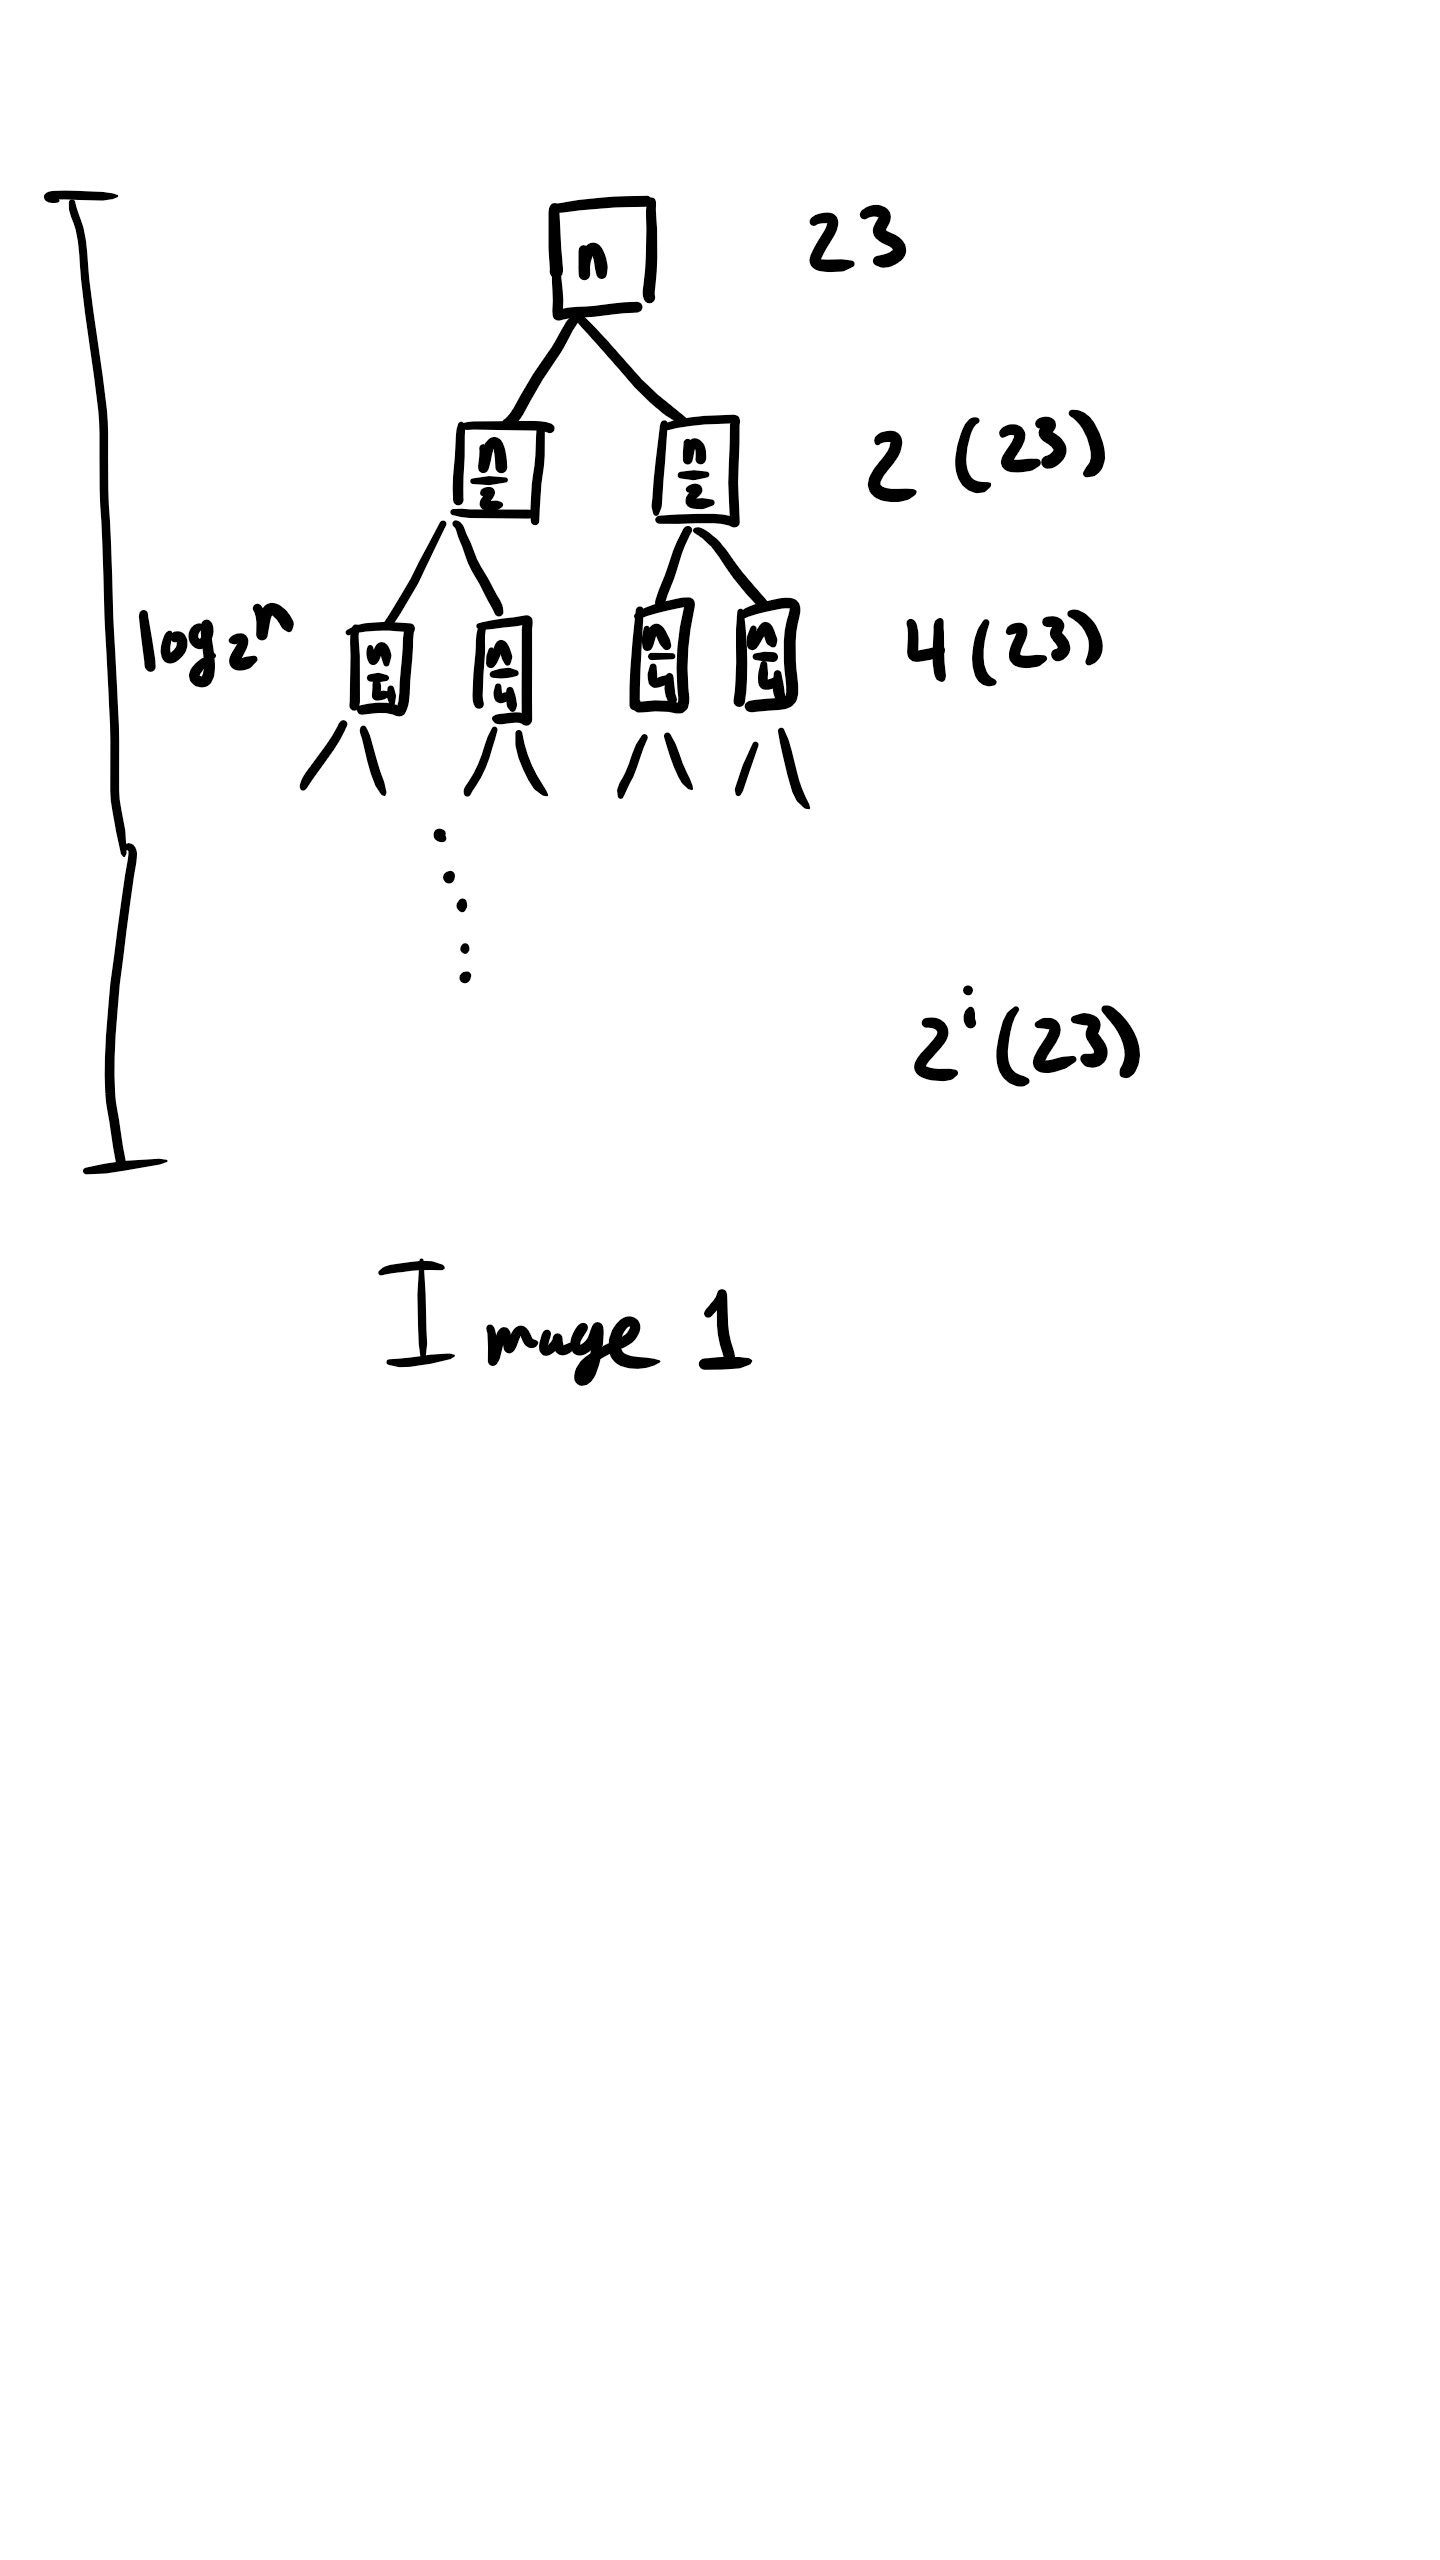
\includegraphics[width=\linewidth]{Image 1.png}
\end{figure}

$$ \sum_{i=0}^{\log_{2}{n}}23\cdot2^i $$
$$ 23\sum_{i=0}^{\log_{2}{n}}2^i $$
$$ \sum_{i=0}^{k}2^i = 2n-1 $$
(Image 1)
Plugging in our bounds we get
$$ T(n) = 23 (2n-1) $$
$$ T(n) = 46n-23 $$
Since we have an explicit formula for the runtime we can see that
$$ T(n) \in \Theta(n) $$

\item [c.] Using the \emph{substitution} method. Make sure to show that the boundary conditions hold as well; choose the constants $c$ and $n_0$ appropriately. \\
We will guess that the function is $O(n)$.
Assume that $T(n') \leq cn'- 25 \quad \forall n' < n$ which gives us
$$ T(n) = 2T(n/2) + 23 $$
$$ T(n) \leq 2\cdot (\frac{cn}{2} - 25) + 23 \leq cn -25$$
$$ T(n) \leq cn - 27 \leq cn - 25 $$
Let $ c = 1$ then we get
$$ T(n) \leq n - 27 \leq n - 25 $$
Which holds true so
$$ T(n) \in O(n) $$

We will also guess that the function is $\Omega (n)$
Assume that $T(n') \geq cn'\quad \forall n' < n$ which gives us
$$ T(n) = 2T(n/2) $$
$$ T(n) \geq 2\cdot (\frac{cn}{2}) + 23 \geq cn $$
$$ T(n) \geq cn + 23 \geq cn $$
Let $ c = 1$ then we get
$$ T(n) \geq n + 23 \geq n $$
Which holds true so
$$ T(n) \in \Omega(n) $$
Since we have shown $O(n)$ and $\Omega(n)$ we have
$$ T(n) \in \Theta(n)$$
\end{itemize}

\section*{Question 2}

For the following algorithm calls, prove a {\em tight} asymptotic bound for their worst-case running time. Pay attention to the input in the algorithm \emph{calls}! \\

\begin{itemize}
\item [a.] The call to \textsc{Recursive-Algorithm}($n$) for some $n>1$.
\vspace{10pt}

\begin{lstlisting}
function Recursive-Algorithm(a):
    q = 0
    if a $\geq$ 1 then
        for i=1 to $\lfloor a \rfloor$ do
            q = q+1
        Recursive-Algorithm(a/2)
        Recursive-Algorithm(a/5)
        Recursive-Algorithm(a/9)
\end{lstlisting}
Going through line by line we can get each runtime
\begin{itemize}
\item [1] $c_{1}$
\item [2] $c_{2}$
\item [3] $c_{3}n$
\item [4] $c_{4}n$
\item [5] $c_{5}T(n/2)$
\item [6] $c_{6}T(n/5)$
\item [6] $c_{6}T(n/9)$
\end{itemize}

We can write the equation describing the runtime as

\begin{equation*}
T(n)=
\begin{cases}
1 &\text{if $n< 1$}\\
T(n/2)+T(n/5)+T(n/9) + O(n) &\text{otherwise.}
\end{cases}
\end{equation*}

We can solve this using a tree (Image 2).
\begin{figure}
    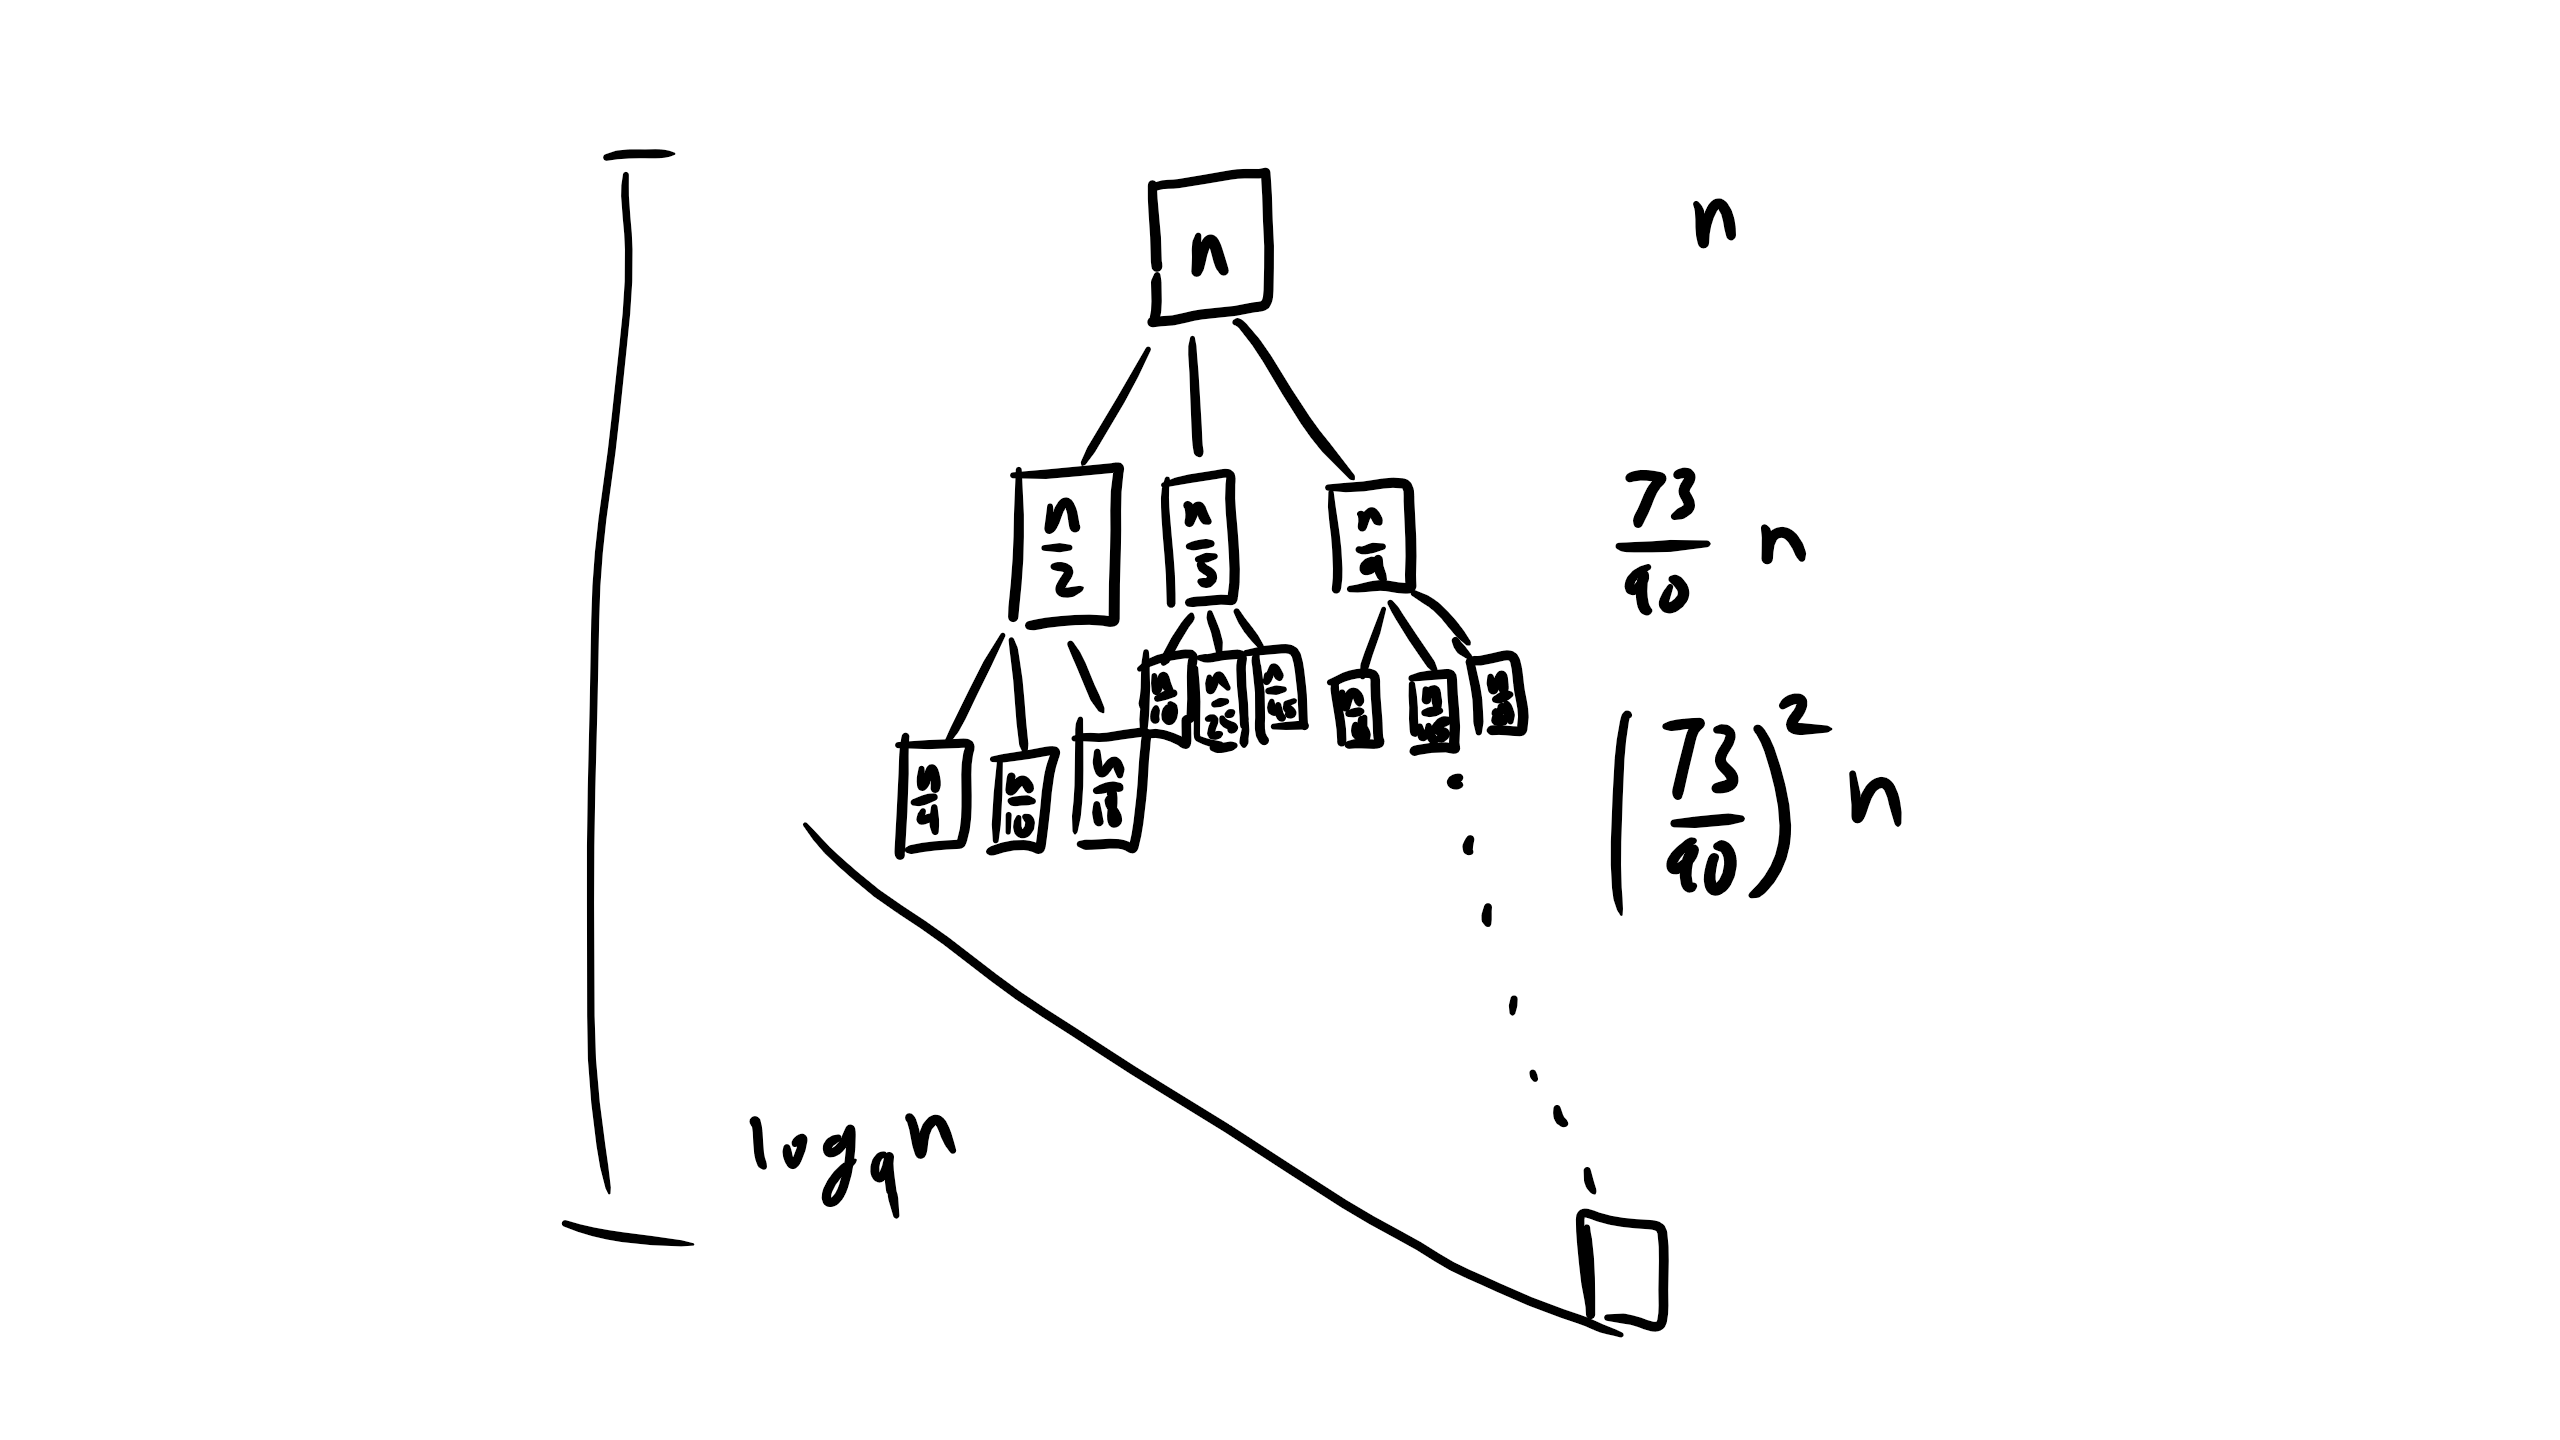
\includegraphics[width=\linewidth]{Image 2.png}
\end{figure}
As we can see in the worst case our tree gives us this result
$$ \sum_{i=0}^{log_{9}{n}}(\frac{73}{90})^in \leq \sum_{i=0}^{\infty}(\frac{73}{90})^in = n\frac{1}{1-\frac{73}{90}} = \frac{90}{17}n $$
Since we over estimated we have shown that at most
$$T(n) \in O(n)$$
But we also know that we will have to do $n$ work on each call so we can't be running faster that $O(n)$. Therefore
$$T(n) \in \Omega(n)$$
Both of these together give us
$$T(n) \in \Theta(n) $$

\item[b.] The call to \textsc{Recursive-Algorithm2}($n,n$) for some $n>2$.

\begin{lstlisting}
function Recursive-Algorithm2(a,b):
    if a $\geq$ 2 and b $\geq$ 2 then
        u = a/3
        v = b-1
        Recursive-Algorithm2(u,v)
\end{lstlisting}
Since we are only looking at Recursive-Algorithm2$(n,n)$ it will run according to this function
\begin{equation*}
T(n,n)=
\begin{cases}
c_{0} &\text{if $n \leq 1$}\\
c_{1}(n-1) &\text{if $ n < \log_{3}{n}$}\\
c_{1}\log_{3}(n) &\text{otherwise}
\end{cases}
\end{equation*}
This is due to the fact that it will stop whenever either repeated division or subtraction reaches 1.
If we find what values of $n$ it switches from one case to the next we get
\begin{equation*}
T(n,n)=
\begin{cases}
c_{0} &\text{if $n \leq 1$}\\
c_{1}\log_{3}(n) &\text{otherwise}
\end{cases}
\end{equation*}
So really the $b$ term will never occur if the input is the same number twice like in our case.
With this we can see that we will fall into $T(n)=c_{1}\log_{3}n$ for our input of $n>2$ so the runtime is
$$ T(n)\in \Theta(\log n) $$

\end{itemize}


\section*{Question 3}
In solving the following recurrence equations, first try to use the master theorem. If it does not apply, explain why this is the case.

\begin{itemize}
\item [a.] Solve the following recurrence equation. \\
\begin{equation*}
T(n) =
\begin{cases}
1 &\text{if $n\leq 1$}\\
T(2n/3)+T(n/4)+\Theta(n) &\text{otherwise.}
\end{cases}
\end{equation*}
We cannot apply the master theorem here as it does not fit the form of
$$T(n) = aT(\frac{n}{b}) + f(n)$$
To solve this recurrence equations we can use substitution or the tree method.
I will proceed with the tree method (Image 3)
\begin{figure}
    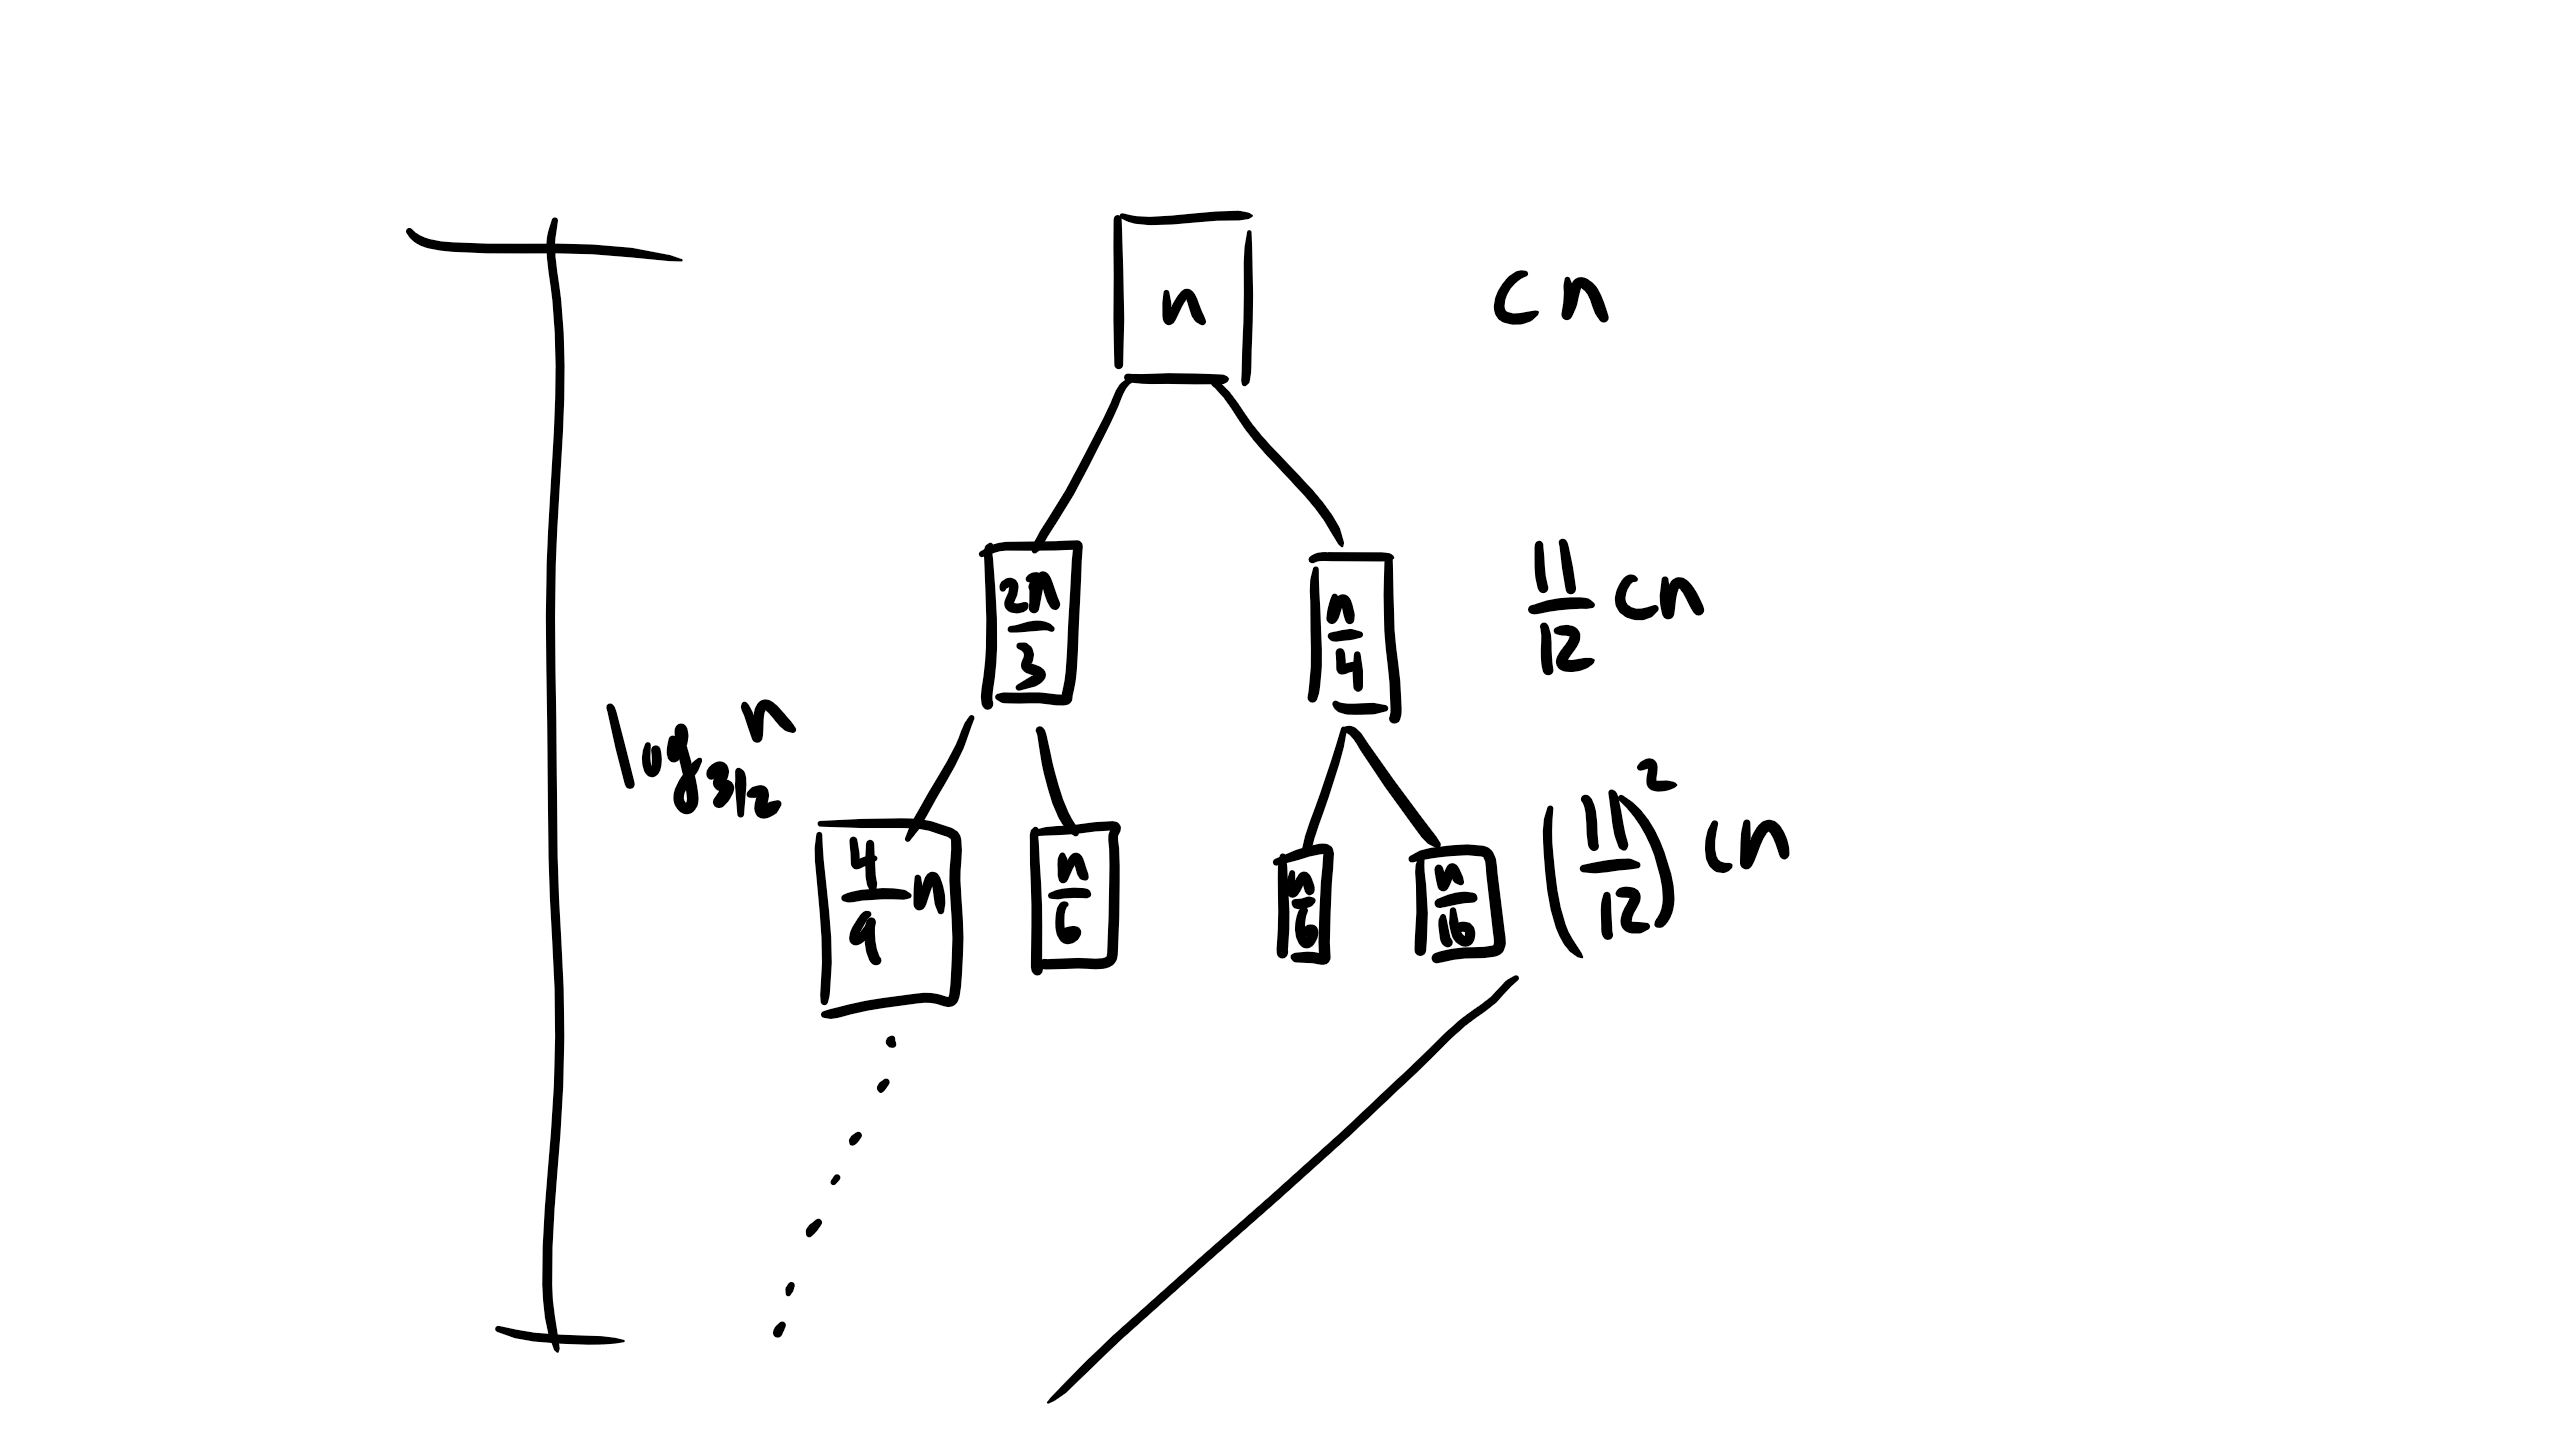
\includegraphics[width=\linewidth]{Image 3.png}
\end{figure}
We can see that each row uses $(\frac{11}{12})^in$ work.
To get an upper bound we can look at the deepest part of the tree which is going to be $\log_{3/2}n$ putting these together we get
$$\sum_{i=0}^{log_{3/2}n}(\frac{11}{12})^in \leq \sum_{i=0}^{\infty}(\frac{11}{12})^in = n\frac{1}{1-\frac{11}{12}} = 12n $$
This gives us an upper bound of $O(n)$
$$ T(n) \in O(n) $$
Since our recurence equation also guarentees that we do at least $\Theta(n)$ then our lower bound is at leas that
$$ T(n) \in \Omega(n)$$
Combining both of these gives us
$$ T(n) \in \Theta(n) $$

\item [b.] Solve the following recurrence equation. \\
\begin{equation*}
T(n) =
\begin{cases}
1 &\text{if $n\leq 1$}\\
4T(n/2)+n^2/\log n &\text{otherwise.}
\end{cases}
\end{equation*}
Applying the master theorem we can find each coefficient to be
$$ a=4 \quad b=2 \quad f(n)=\frac{n^2}{\log{n}}$$
$$ \log_{2}{4}=2 $$
No case of the master theorem applies since
$$f(n)\notin O(n^{2-\epsilon}) \quad f(n)\notin \Theta(n^2) \quad f(n)\notin \Omega(n^{2+\epsilon})$$
So we must continue using either the tree method or substitution.
I will proceed with the tree method (Image 4)
\begin{figure}
    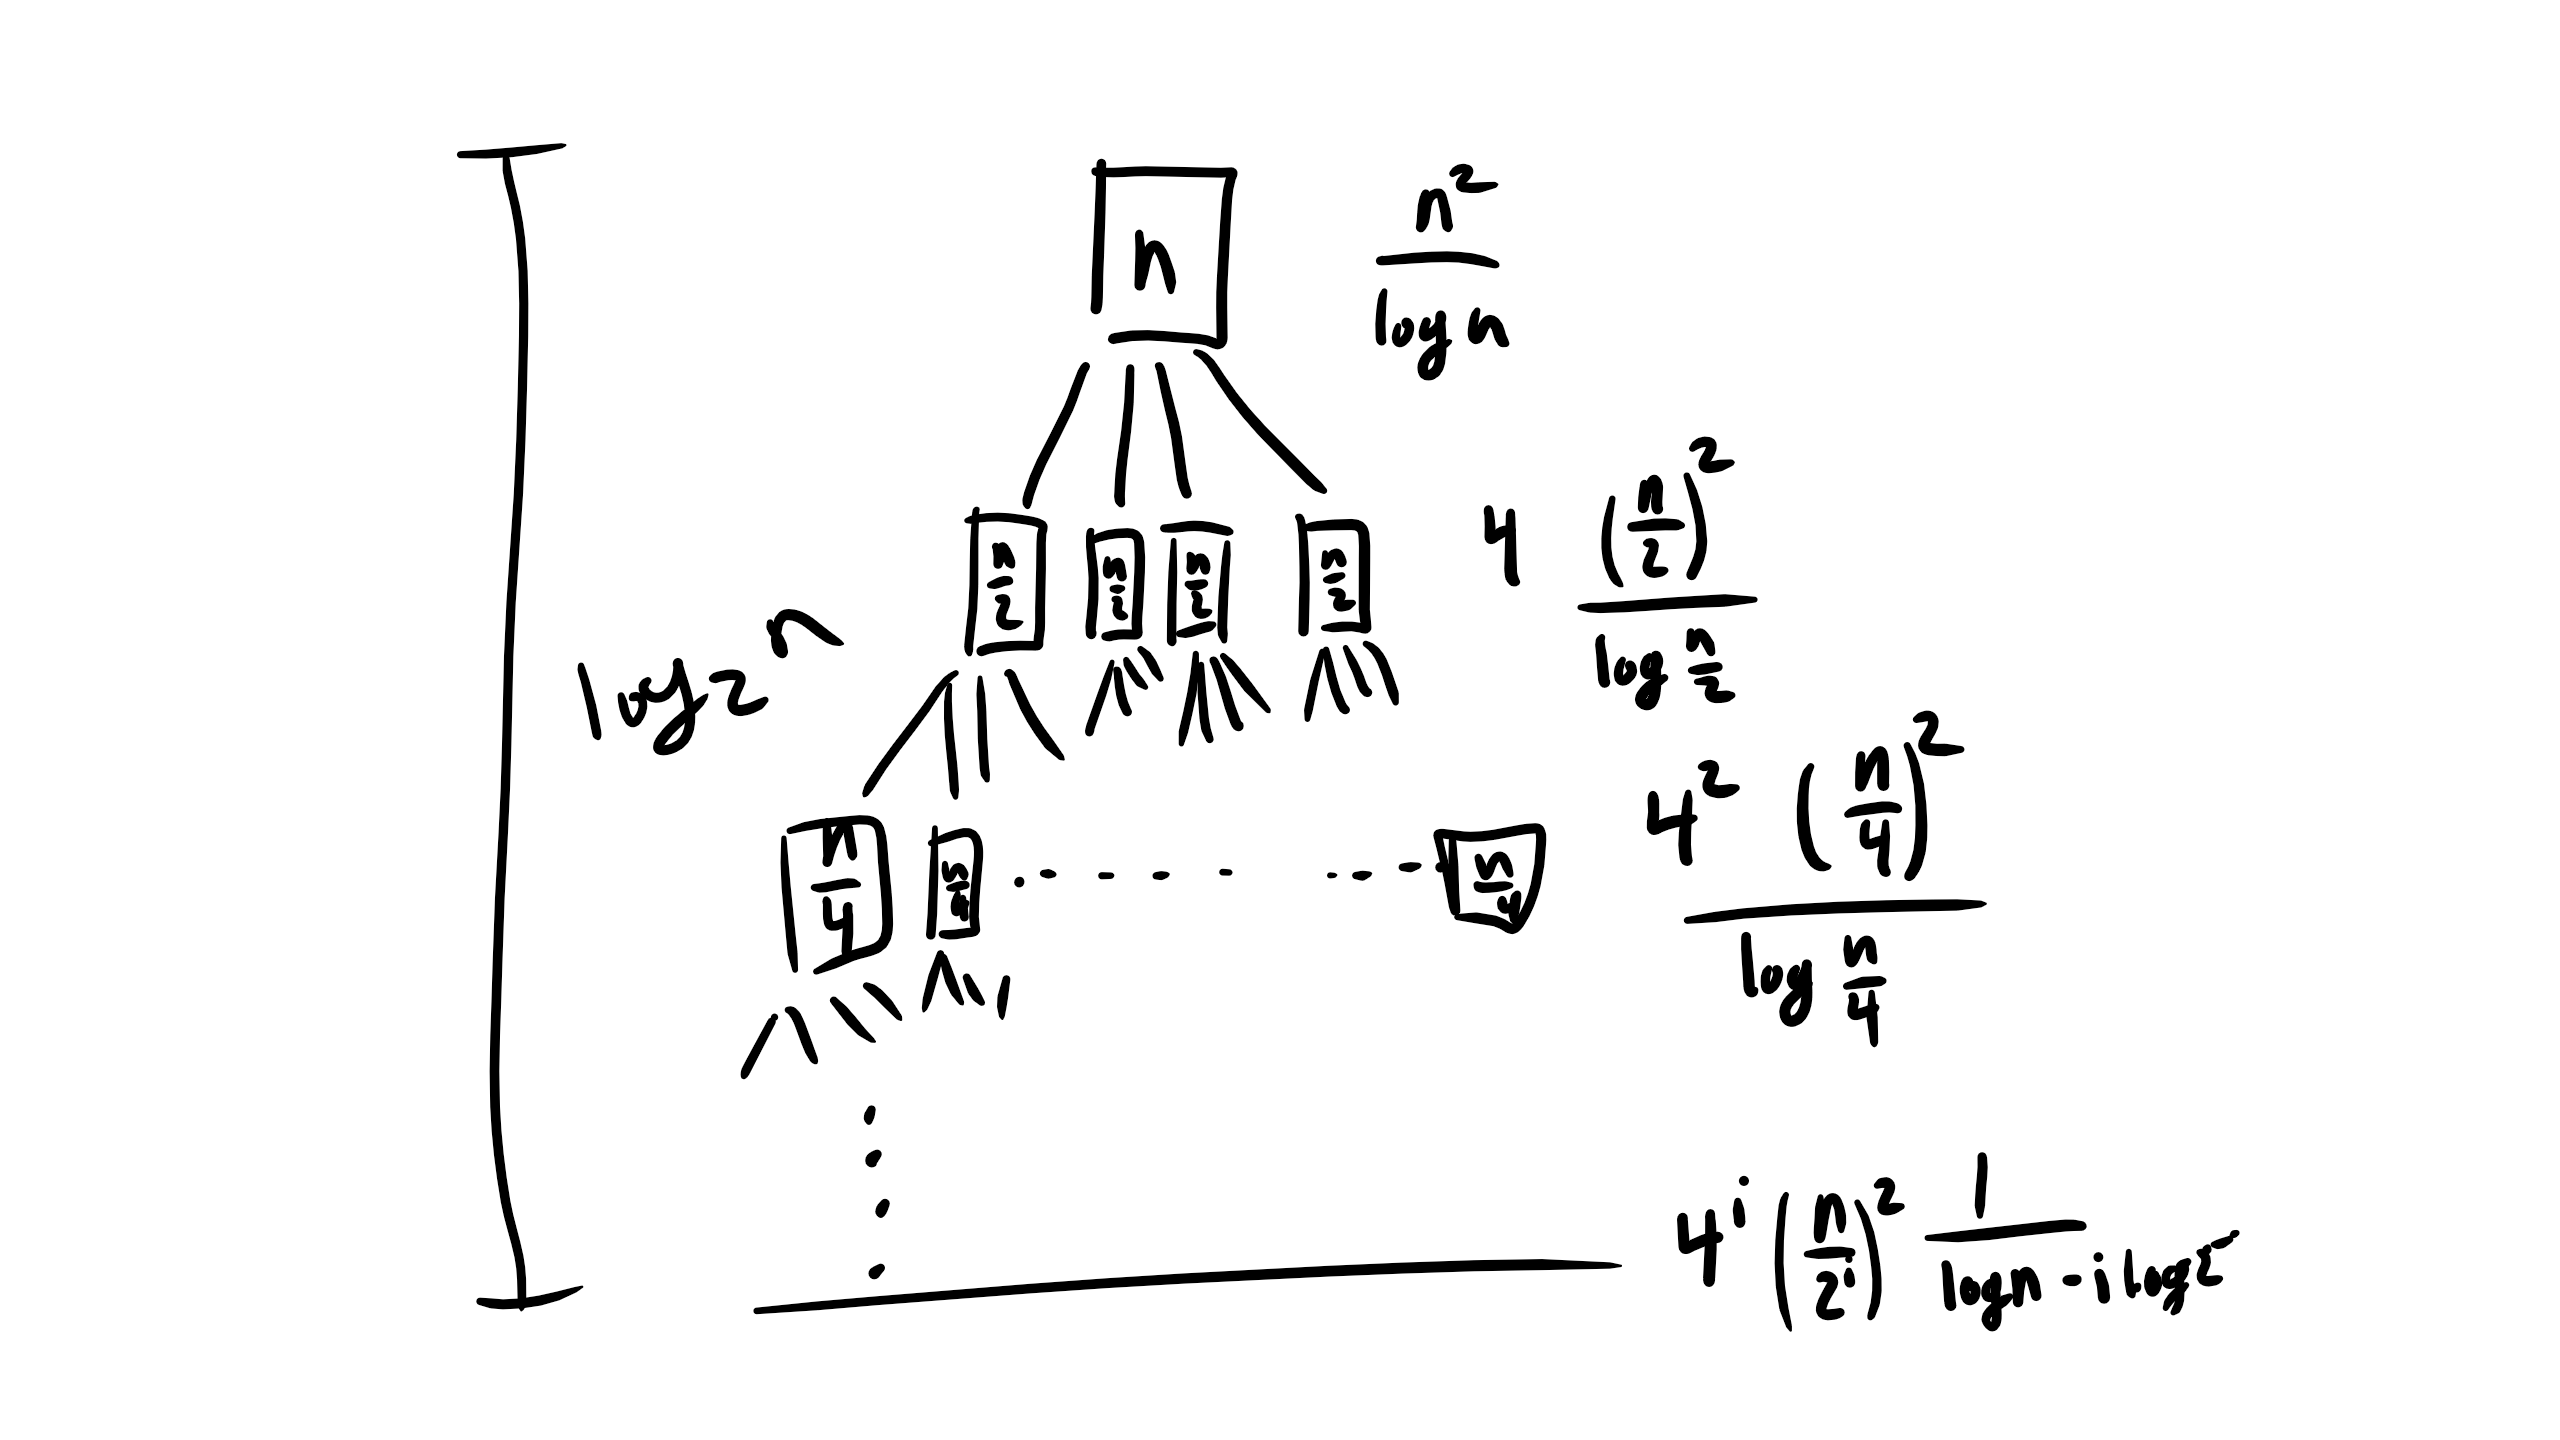
\includegraphics[width=\linewidth]{Image 4.png}
\end{figure}
We can see each row uses
$$4^i \frac{(\frac{n}{2^i})^2}{\log_{2}{\frac{n}{2^i}}}$$
We can also see the depth is given by $\log_{2}{n}$ which gives us
$$ \sum_{i=0}^{\log_{2}{n}} 4^i \frac{(\frac{n}{2^i})^2}{\log_{2}{\frac{n}{2^i}}} =
n^2 \sum_{i=0}^{\log_{2}{n}} \frac{1}{(\log_{2}{n} - i)} $$
Our denominator is just counting from up to down so we can get the same result if we count from down to up
$$ n^2 \sum_{i=0}^{\log_{2}{n}} \frac{1}{i} $$
In our denominator we have a Harmonic series which we know grows like $\log{n}$ so we have
$$n^2 \sum_{i=0}^{\infty} \frac{1}{i} \in n^2\log\log{n} $$
$$ T(n) \in n^2\log\log{n} $$



\item [c.] For the following equation provide an exact (\emph{not asymptotic}) closed form solution. \\
\begin{equation*}
T(n) =
\begin{cases}
1 &\text{if $n\leq 1$}\\
5T(n/2) &\text{otherwise.}
\end{cases}
\end{equation*}
We can solve this explicitly with repeated substitution
$$\text{zero iterations} \quad T(n) = 5T(\frac{n}{2})$$
$$\text{first iteration} \quad T(n) = 5(5T(\frac{n}{4}))$$
$$\text{second iteration} \quad T(n) = 5(5(5T(\frac{n}{16})))$$
$$\text{i'th iterations} \quad T(n) = 5^iT(\frac{n}{2^i}))$$
Which will hit the "base case" after $\lfloor \log_{2}n \rfloor$ iterations so
$$ T(n) = 5^{\lfloor \log_{2}n \rfloor} $$
\end{itemize}

\section*{Question 4}
Consider the following variation of Merge Sort: rather than dividing the array into
two equal sized parts, recursively sorting each of them, and then merging them together, we divide
the array into $\sqrt{n}$ equal sized parts instead. Once we recursively sort each one of these
$\sqrt{n}$ parts of size $\sqrt{n}$ each, we need $\Theta(n\lg n)$ time in order to merge them together,
leading to the following recurrence equation:
\begin{equation*}
T(n)=
\begin{cases}
1 &\text{if $n\leq 1$}\\
\sqrt{n}T(\sqrt{n})+n\lg n &\text{otherwise.}
\end{cases}
\end{equation*}
Solve this recurrence equation, providing tight upper and lower bounds
\begin{itemize}
\item [a.] Using the \emph{recursion tree} method.
\begin{figure}
    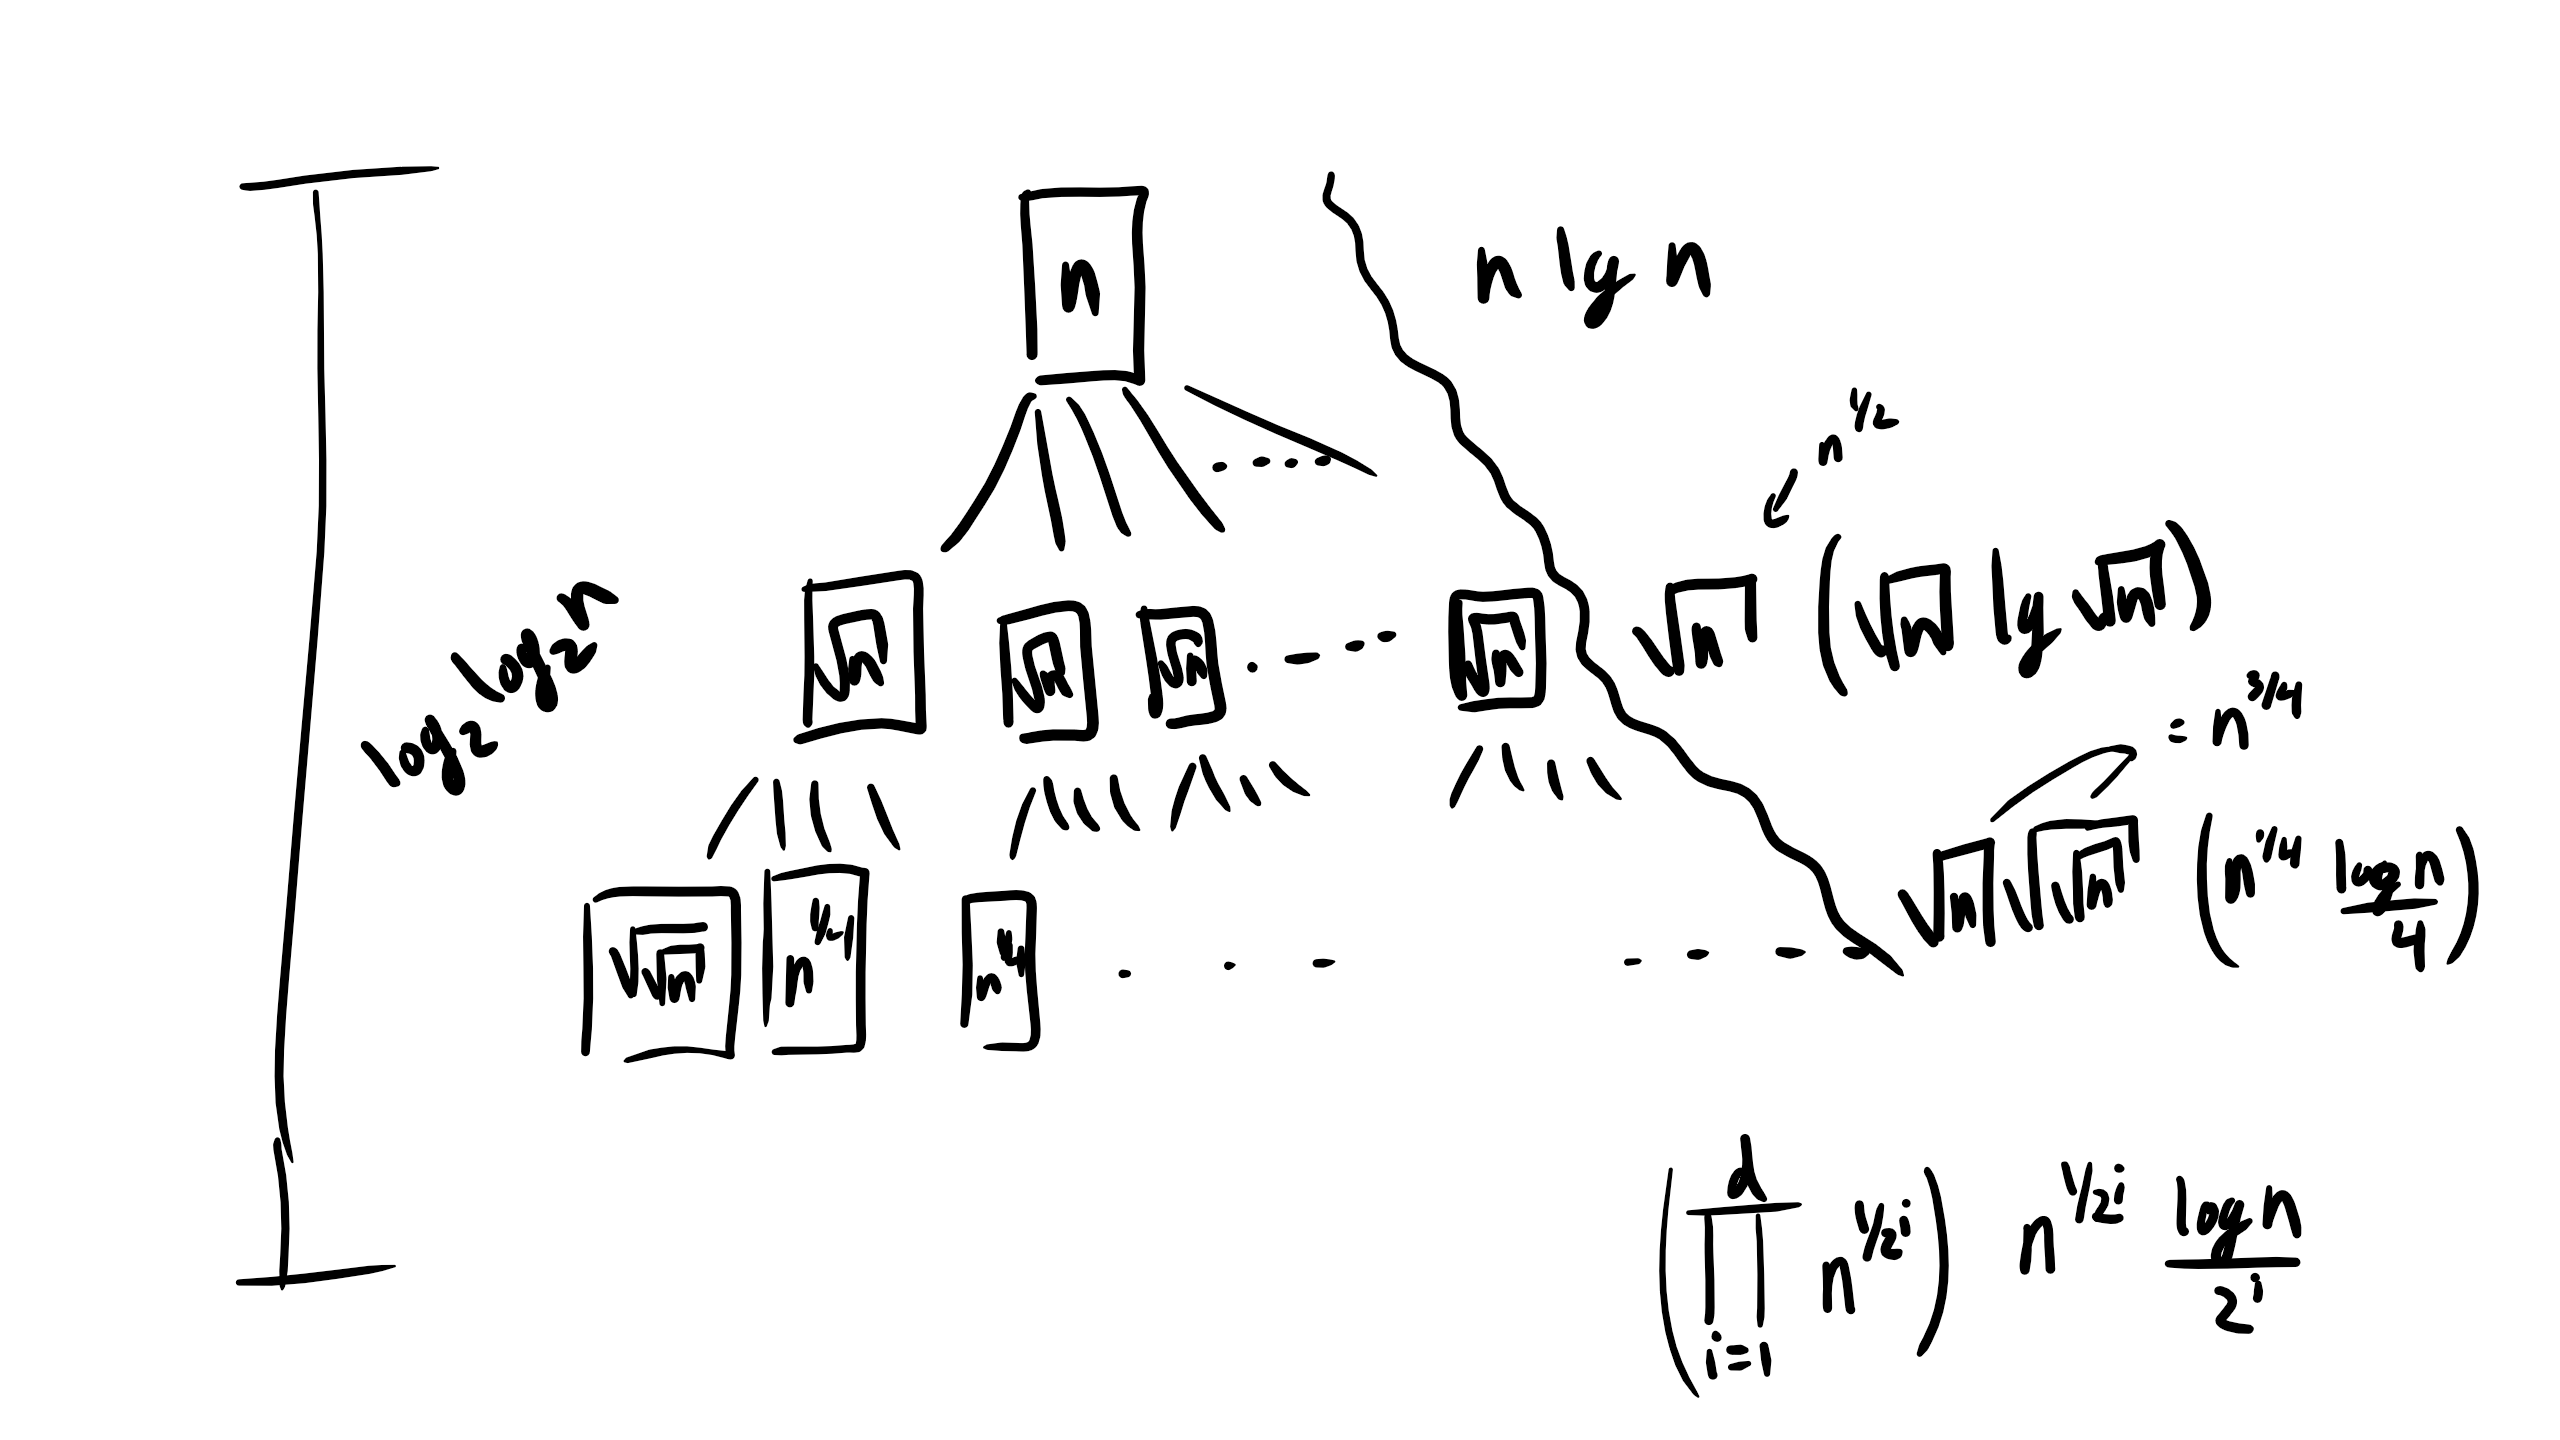
\includegraphics[width=\linewidth]{Image 5.png}
\end{figure}
(Image 5)We can see that each node has a cost of $n^{\frac{1}{2^i}}\log_{2}{n^{\frac{1}{2^i}}}$ and on each level there are $\Pi_{i=1}^{d}n^{\frac{1}{2^i}}$
Which can be rewritten as
$$ n^{1-\frac{1}{2^{d}}} $$
The only exception appears to be the first level so this equation holds for $d > 0 $
The height of the tree can be solved by finding this solution
$$ n^{\frac{1}{2^i}} = 2$$
$$ \frac{1}{2^i} \log{n} = \log{2} $$
$$ 2^i = \frac{\log{n}}{\log{2}} $$
$$ i = \log_{2}{{\log_{2}{n}}}$$
So our total cost can be given by
$$ T(n) = n\log_{2}{n} + \sum_{1}^{\log_{2}{\log_{2}{n}}} n^{1-\frac{1}{2^{i}}}(n^{\frac{1}{2^i}}\log_{2}{n^{\frac{1}{2^i}}})$$
$$ T(n) = n\log_{2}{n} + \sum_{1}^{\log_{2}{\log_{2}{n}}} n\frac{\log_{2}{n}}{2^i}$$
$$ T(n) = n\log_{2}{n} + n\log_{2}{n}\sum_{1}^{\log_{2}{\log_{2}{n}}} \frac{1}{2^i}$$
$$ T(n) \leq n\log_{2}{n} + n\log_{2}{n}\sum_{1}^{\infty} \frac{1}{2^i}$$
$$ T(n) \leq n\log_{2}{n} + n\log_{2}{n}\sum_{1}^{\infty} \frac{1}{2^i}$$
$$ T(n) \leq 2n\log_{2}{n} $$
$$ T(n) \in O(n\log{n})$$
Since we know we have to at least do $n\log{n}$ work we also know that
$$ T(n) \in \Omega(n\log{n})$$
Therefore
$$ T(n) \in \Theta(n\log{n})$$

\item [b.] Using the \emph{master theorem} after applying an appropriate change of variables.
$$ T(n) = \sqrt{n}T(\sqrt{n})+n\log{n} $$
Let $ m = \log{n} \implies n=2^m $
$$ T(2^m) = 2^{\frac{m}{2}}T(2^{\frac{m}{2}}) +m2^m $$
Let $ S(m) = \frac{T(2^m)}{2^m} $
$$ S(m) = S(\frac{m}{2}) + m $$
Now applying the master theorem we get
$$ a = 1 \qquad b = 2 \qquad f(n)=n \qquad \log_{2}{1} = 0 $$
We can apply the third case of the master theorem, if we let $\epsilon = .5$ we have
$$ m \in \Omega(\sqrt{m}) $$
Taking $ c = .9 $ we can see
$$f(\frac{m}{2}) \leq .9f(m) \implies \frac{m}{2} \leq .9m $$
By the master theorem we know that
$$ S(m) \in \Theta(m) $$
Substituting backwards we get
$$ T(2^m) \in \Theta(m2^m) $$
$$ T(n) \in \Theta(n\log{n}) $$

\end{itemize}

\end{document}
